\section{1174096 - Nico Ekklesia Sembiring}
\subsection{Soal Teori}
\begin{enumerate}

	\item Jelaskan kenapa kata-kata harus di lakukan vektorisasi
	\hfill\break
	Kata kata harus dilakukan vektorisasi dikarenakan atau bertujuan utk mengukur nilai kemunculan suatau kata yang serupa dari sebuah kalimat sehingga kata-kata tersebut dapat di prediksi kemunculanya. atau juga di buatnya vektorisasi data digunakan untuk memprediksi bobot dari suatu kata misalkan ayam dan kucing sama-sama hewan maka akan dibuat prediksi apakah kata tersebut akan muncul pada kalimat yang kira-kira memiliki bobot yang sama.
	
    \begin{figure}[H]
	\centering
		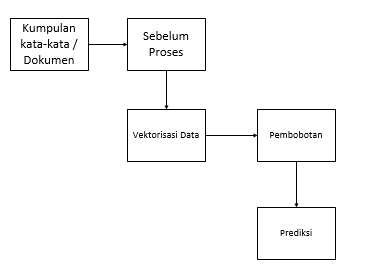
\includegraphics[width=4cm]{figures/1174096/tugas5/1-1.PNG}
		\caption{Ilustrasi vektorisasi.}
	\end{figure}

	\item Jelaskan mengapa dimensi dari vektor dataset google bisa sampai 300
	\hfill\break
    Dimensi dataset dari google bisa mencapai 300 karena dimensi dari vektor tersebut digunakan untuk membandingkan bobot dari setiap kata, misalkan terdapat kata dog dan cat pada dataset google tersebut setiap kata tersebut di buat dimensi vektor 300 untuk kata dog dan 300 dimensi vektor juga untuk kata cat kemudian kata tersebt di bandingkan bobot kesamaan katanya maka akan muncul akurasi sekitar 70 persen kesamaan bobot dikarenakan kata dog dan cat sama sama di gunakan untuk hewan peliharaan.
	
    \begin{figure}[H]
	\centering
		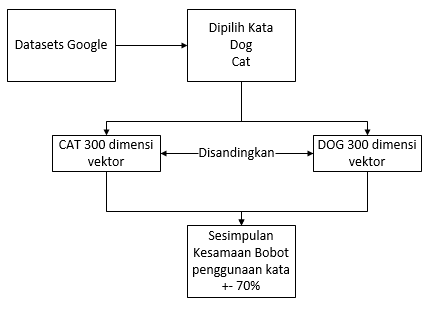
\includegraphics[width=4cm]{figures/1174096/tugas5/1-2.PNG}
		\caption{ilustrasi dataset google.}
	\end{figure}


	\item Jelaskan konsep vektorisasi untuk kata
	\hfill\break
	Vektorisasi untuk kata untuk mengetahui kata tengah dari suatau kalimat atau kata utama atau objek utama pada suatau kalimat contoh ( Jangan lupa subscribe channel saya ya sekian treimakasih ) kata tengah tersebut merupakan channel yang memiliki bobot sebagai kata tengah dari suatu kalimat atau bobot sebagai objek dari suatu kalimat. hal ini sangat berkaitan dengan dimensi vektor pada dataset google yang 300 tadi karena untuk mendapatkan nilai atau bobot dari kata tengah tersebut di dapatkan dari proses dimensiasi dari kata tersebut. 
    \begin{figure}[H]
	\centering
		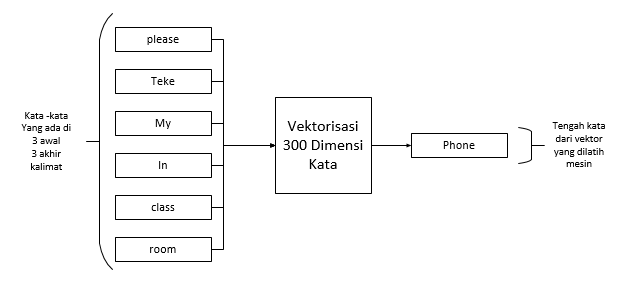
\includegraphics[width=4cm]{figures/1174096/tugas5/1-3.PNG}
		\caption{Ilustrasi konsep vektorisasi untuk kata.}
	\end{figure}

	\item Jelaskan konsep vektorisasi untuk dokumen.
	\hfill\break
	Vektorisasi untuk dokumen hampir sama seperti vektorisasi untuk kata hanya saja pemilihan kata utama atau kata tengah terdapat pada satu dokumen jadi mesin akan membuat dimensi vektor 300 untuk dokumen dan nanti kata tengahnya akan di sandingkan pada dokumen yany terdapat pada dokumen tersebut.
    \begin{figure}[H]
	\centering
		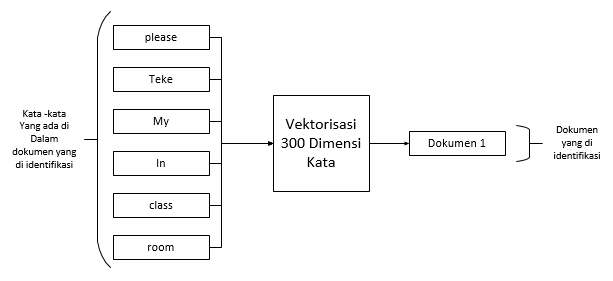
\includegraphics[width=4cm]{figures/1174096/tugas5/1-4.PNG}
		\caption{Ilustrasi konsep vektorisasi untuk dokumen.}
	\end{figure}

	\item Jelaskan apa mean dan standar deviasi.
	\hfill\break
	Mean merupakan petunjuk terhadap kata-kata yang di olah jika kata kata itu akurasinya tinggi berarti kata tersebut sering muncul begitu juga sebaliknya, sedangkan setandar defiation merupakan standar untuk menimbang kesalahan. sehingga kesalahan tersebut di anggap wajar misarkan kita memperkirakan kedalaman dari dataset merupakan 2 atau 3 tapi pada kenyataanya merupakan 5 itu merupakan kesalahan tapi masih bisa dianggap wajar karna masih mendekati perkiraan awal.
	\begin{figure}[H]
	\centering
		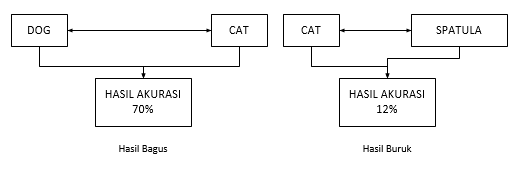
\includegraphics[width=4cm]{figures/1174096/tugas5/1-5.PNG}
		\caption{Ilustrasi mean dan standar deviasi.}
	\end{figure}

	\item Jelaskan apa itu skip-gram
	\hfill\break
	Skip-Gram adalah kebalikan dari konsep vektorisasi untuk kata dimana kata tengah menjadi acuan terhadap kata kata pelengkap dalam suatu kalimat.

	\begin{figure}[H]
	    \centering
	    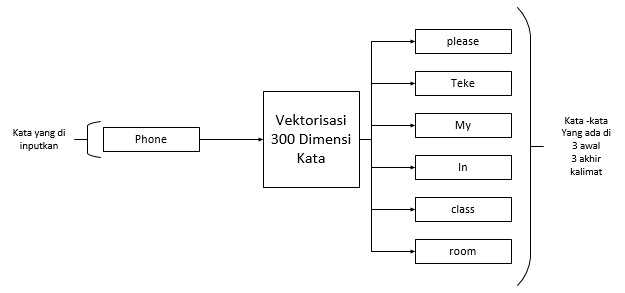
\includegraphics[width=4cm]{figures/1174096/tugas5/1-6.PNG}
	    \caption{Ilustrasi skipgram.}
	\end{figure}
\end{enumerate}
\subsection{Praktek}
\begin{enumerate}
    \item Cobalah dataset google, dan jelaskan vektor dari kata love, faith, fall, sick, clear, shine, bag, car, wash, motor, cycle dan cobalah untuk melakukan perbandingan similirati dari masing-masing kata tersebut. jelaskan arti dari outputan similaritas dan setiap baris kode yang dibuat
    \begin{itemize}
        \item berikut adalah hasil dari code yang digunakan untuk memanggil data library GENSIM dengan menggunakan perintah import, lalu dari library tersebut diambillah data yang akan digunakan untuk memproses data dari GoogleNews-vector. ilustrasi dapat dilihat pada gambar
        \begin{figure}[H]
            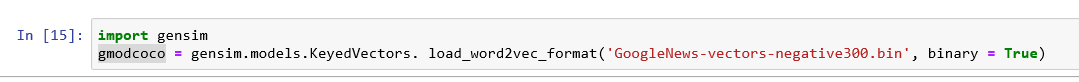
\includegraphics[width=4cm]{figures/1174096/tugas5/praktek1-1.PNG}
            \centering
            \caption{import gensim dan olah data GoogleNews-vector}
        \end{figure}
        
        \item lalu pada penggunaan code berikut ini akan mengolah data LOVE yang terdapat pada file GoogleNews-vector, hasil dari pemrosesannya dapat dilihat pada gambar
        \begin{figure}[H]
            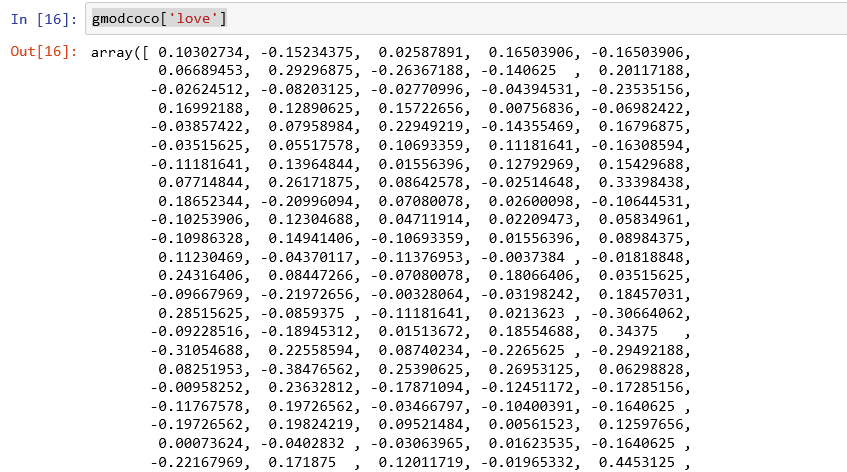
\includegraphics[width=4cm]{figures/1174096/tugas5/praktek1-2.PNG}
            \centering
            \caption{hasil olah data LOVE pada GoogleNews-vector}
        \end{figure}
        
        \item  lalu pada penggunaan code berikut ini akan mengolah data FAITH yang terdapat pada file GoogleNews-vector, hasil dari pemrosesannya dapat dilihat pada gambar
        \begin{figure}[H]
            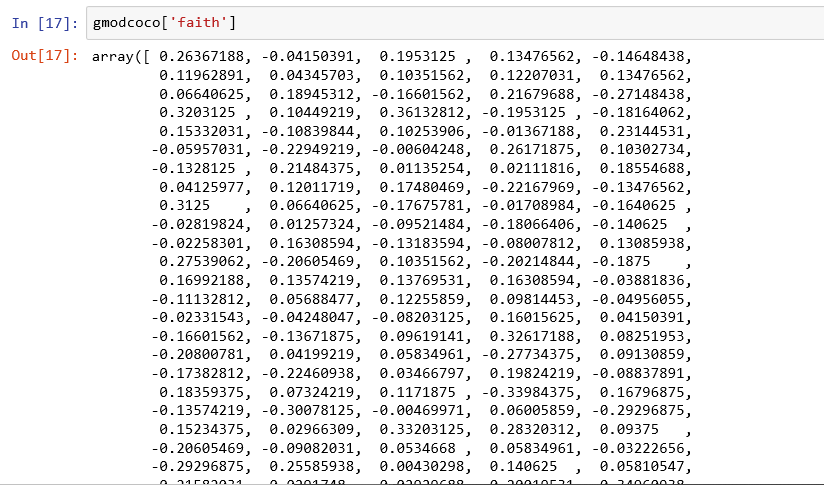
\includegraphics[width=4cm]{figures/1174096/tugas5/praktek1-3.PNG}
            \centering
            \caption{hasil olah data FAITH pada GoogleNews-vector}
        \end{figure}
        
        \item  lalu pada penggunaan code berikut ini akan mengolah data FALL yang terdapat pada file GoogleNews-vector, hasil dari pemrosesannya dapat dilihat pada gambar
        \begin{figure}[H]
            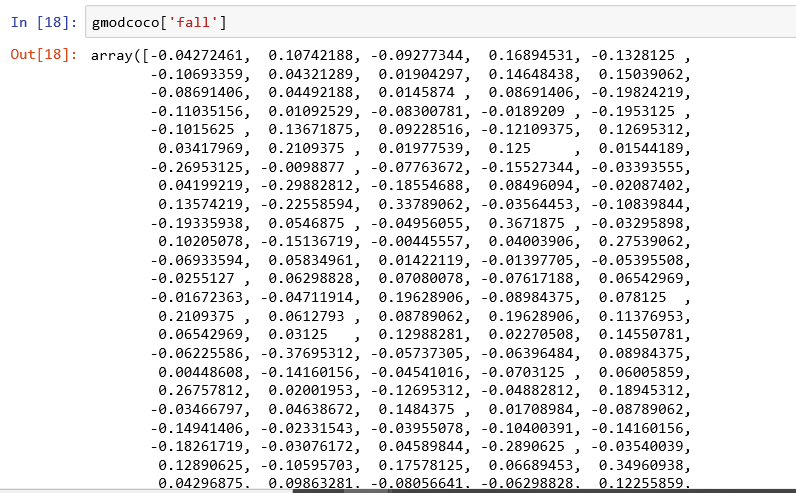
\includegraphics[width=4cm]{figures/1174096/tugas5/praktek1-4.PNG}
            \centering
            \caption{hasil olah data FALL pada GoogleNews-vector}
        \end{figure}
        
        \item  lalu pada penggunaan code berikut ini akan mengolah data SICK yang terdapat pada file GoogleNews-vector, hasil dari pemrosesannya dapat dilihat pada gambar
        \begin{figure}[H]
            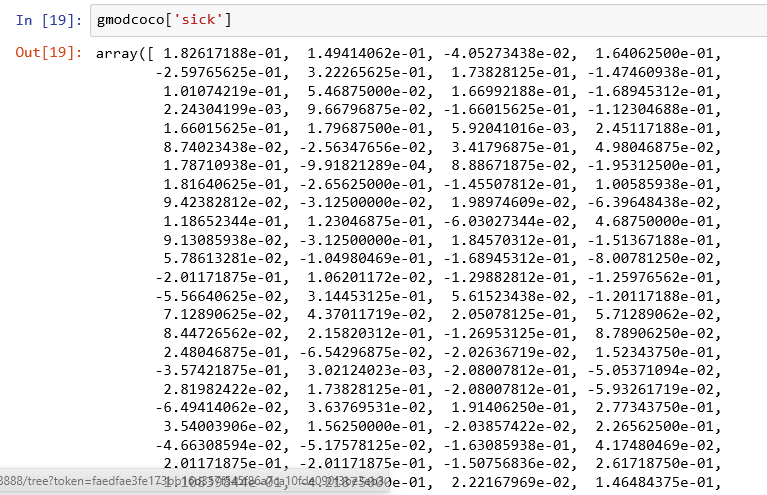
\includegraphics[width=4cm]{figures/1174096/tugas5/praktek1-5.PNG}
            \centering
            \caption{hasil olah data SICK pada GoogleNews-vector}
        \end{figure}
        
        \item  lalu pada penggunaan code berikut ini akan mengolah data CLEAR yang terdapat pada file GoogleNews-vector, hasil dari pemrosesannya dapat dilihat pada gambar
        \begin{figure}[H]
            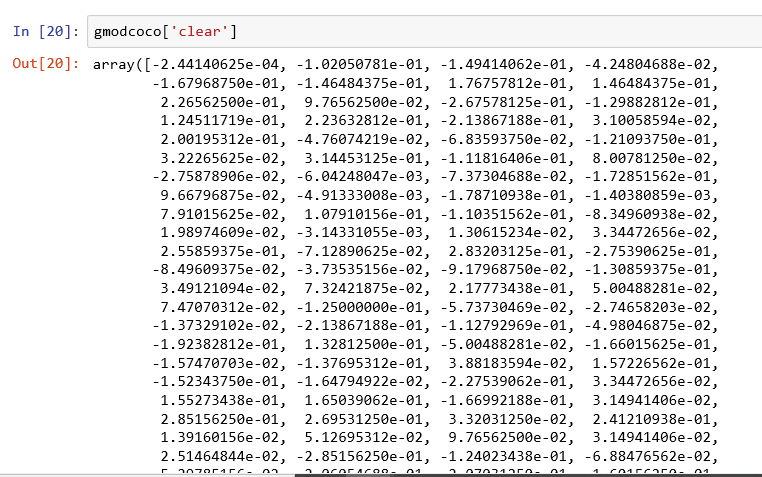
\includegraphics[width=4cm]{figures/1174096/tugas5/praktek1-6.PNG}
            \centering
            \caption{hasil olah data CLEAR pada GoogleNews-vector}
        \end{figure}
        
        \item  lalu pada penggunaan code berikut ini akan mengolah data SHINE yang terdapat pada file GoogleNews-vector, hasil dari pemrosesannya dapat dilihat pada gambar
        \begin{figure}[H]
            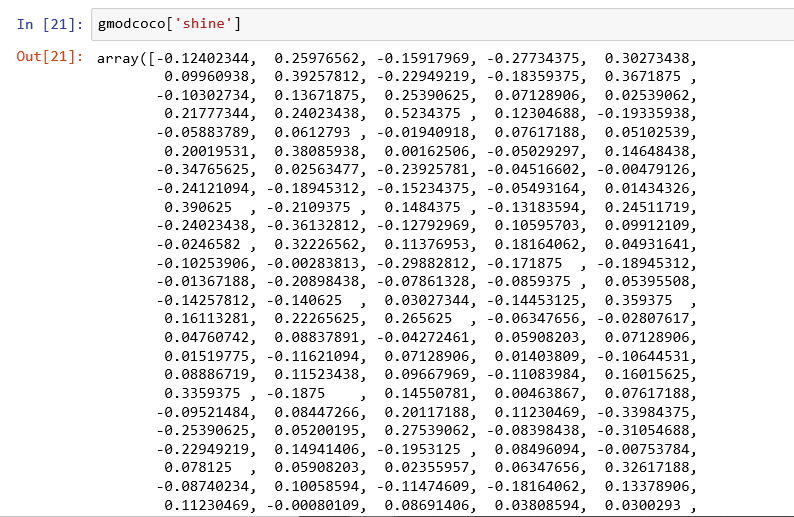
\includegraphics[width=4cm]{figures/1174096/tugas5/praktek1-7.PNG}
            \centering
            \caption{hasil olah data SHINE pada GoogleNews-vector}
        \end{figure}
        
        \item  lalu pada penggunaan code berikut ini akan mengolah data BAG yang terdapat pada file GoogleNews-vector, hasil dari pemrosesannya dapat dilihat pada gambar
        \begin{figure}[H]
            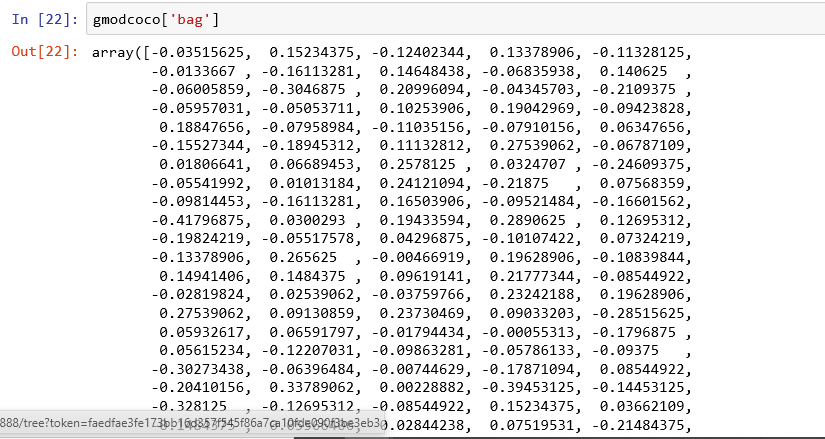
\includegraphics[width=4cm]{figures/1174096/tugas5/praktek1-8.PNG}
            \centering
            \caption{hasil olah data BAG pada GoogleNews-vector}
        \end{figure}
        
        \item  lalu pada penggunaan code berikut ini akan mengolah data CAR yang terdapat pada file GoogleNews-vector, hasil dari pemrosesannya dapat dilihat pada gambar
        \begin{figure}[H]
            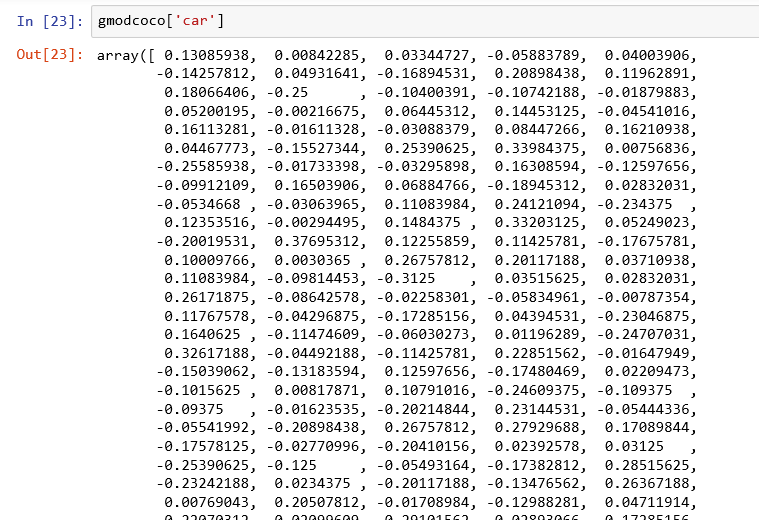
\includegraphics[width=4cm]{figures/1174096/tugas5/praktek1-9.PNG}
            \centering
            \caption{hasil olah data CAR pada GoogleNews-vector}
        \end{figure}
        
        \item  lalu pada penggunaan code berikut ini akan mengolah data WASH yang terdapat pada file GoogleNews-vector, hasil dari pemrosesannya dapat dilihat pada gambar
        \begin{figure}[H]
            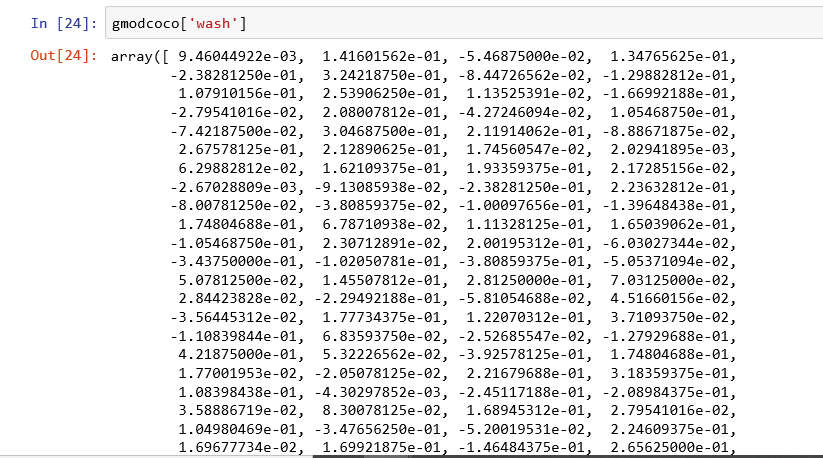
\includegraphics[width=4cm]{figures/1174096/tugas5/praktek1-10.PNG}
            \centering
            \caption{hasil olah data WASH pada GoogleNews-vector}
        \end{figure}
        
        \item  lalu pada penggunaan code berikut ini akan mengolah data MOTOR yang terdapat pada file GoogleNews-vector, hasil dari pemrosesannya dapat dilihat pada gambar 
        \begin{figure}[H]
            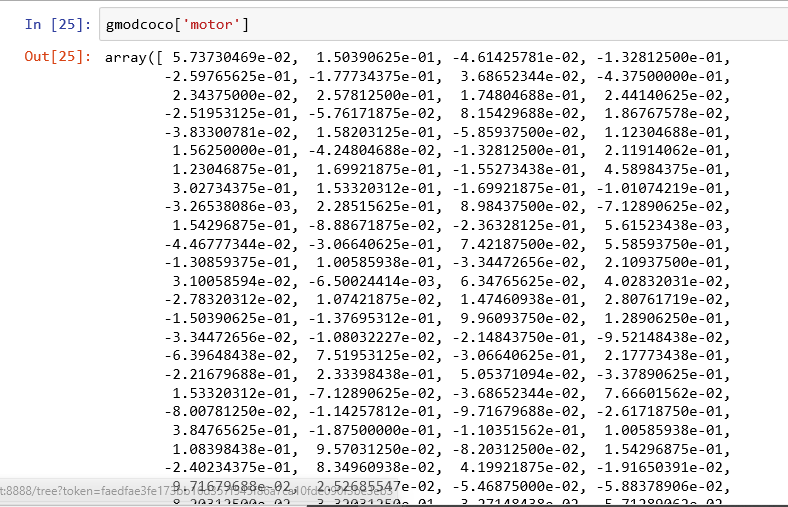
\includegraphics[width=4cm]{figures/1174096/tugas5/praktek1-11.PNG}
            \centering
            \caption{hasil olah data MOTOR pada GoogleNews-vector}
        \end{figure}
        
        \item  lalu pada penggunaan code berikut ini akan mengolah data CYCLE yang terdapat pada file GoogleNews-vector, hasil dari pemrosesannya dapat dilihat pada gambar
        \begin{figure}[H]
            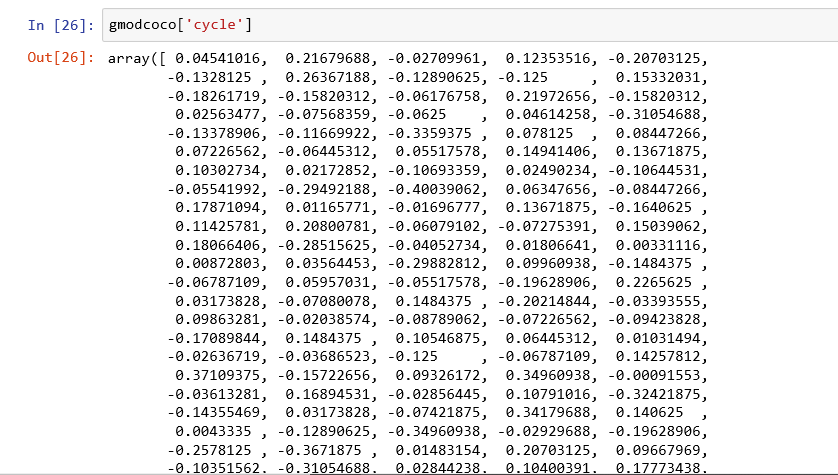
\includegraphics[width=4cm]{figures/1174096/tugas5/praktek1-12.PNG}
            \centering
            \caption{hasil olah data CYCLE pada GoogleNews-vector}
        \end{figure}
        
        \item  dan pada hasil code berikut ini adalah hasil dari proses penggunaan perintah code similarity yang akan menghitung nilai value data yang dibandingkan dengan masing - masing kata seperti pada hasil dari perbandingan kata LOVE disandingkan dengan FAITH menghasilkan nilai 37 persen, sedangkan kata WASH dan SHINE menghasilkan nilai 27 persen dan kata CAR yang disandingkan dengan kata MOTOR menghasilkan 48 persen, dimana kita dapat menyimpulkan bahwa semakin data kata tersebut memiliki tingkat kesamaan yang tinggi maka nilai hasil yang ditampilkanpun akan semakin tinggi. ilustrasi bisa dilihat pada gambar
        \begin{figure}[H]
            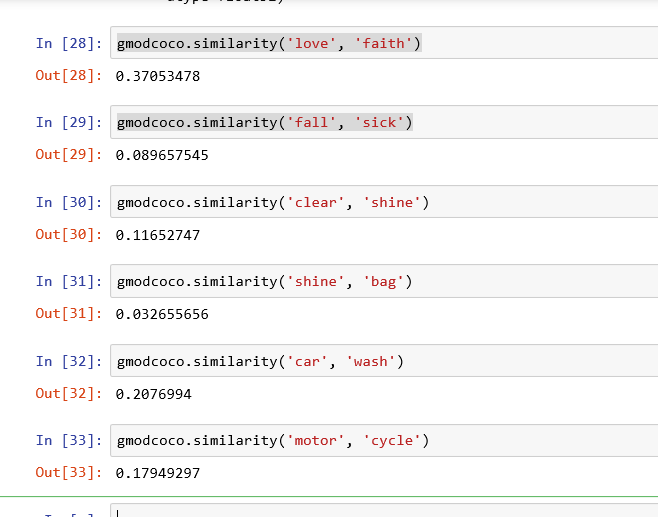
\includegraphics[width=4cm]{figures/1174096/tugas5/praktek1-13.PNG}
            \centering
            \caption{hasil olah data  pada GoogleNews-vector menggunakan SIMILARITY}
        \end{figure}
    \end{itemize}
    
    \item Jelaskan dengan kata dan ilustrasi fungsi dari extract words dan PermuteSentences
    Pada penjelasan berikut ini akan menyangkut pembersihan data yang akan digunakan untuk diproses, dimana data akan di EXTRACT dari setiap katanya agar terbebas dari data TAG HTML, APOSTROPHES, TANDA BACA, dan SPASI yang berlebih. dengan menggunakan perintah code STRIP dan SPLIT. lalu penggunaan library random yang akan dibuat untuk melakukan KOCLOK data dengan acuan datanya adalah data yang terdapat pada variable KATA. untuk ilustrasi hasil dari codenya dapat dilihat pada gambar
    \begin{figure}[H]
        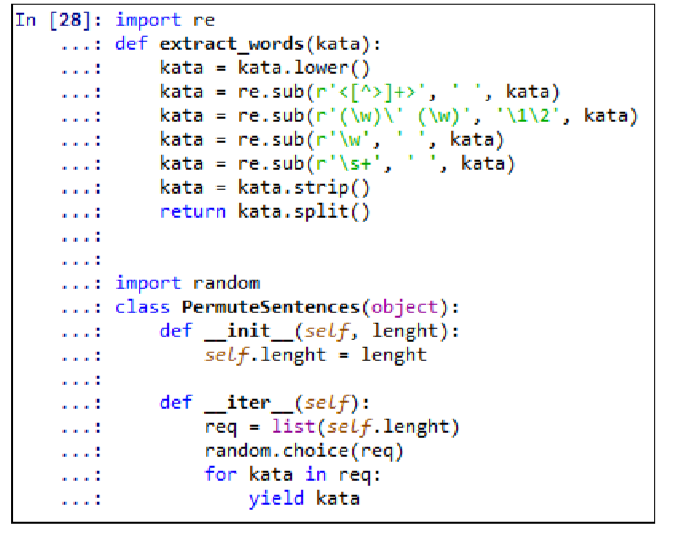
\includegraphics[width=4cm]{figures/1174096/tugas5/praktek2.PNG}
        \centering
        \caption{extract word dan permutesentences}
    \end{figure}

    \item Jelaskan fungsi dari librari gensim TaggedDocument dan Doc2Vec 
    Gensim merupakan open-source model ruang vektor dan toolkit topic modeling, yang diimplementasikan dalam bahasa pemrograman Python. Untuk kinerja Gensim, digunakan NumPy, SciPy dan Cython (opsional). Gensim secara khusus ditujukan untuk menangani koleksi teks besar dengan menggunakan algoritma secara online. Gensim mengimplementasikan tf-idf, latent semantic analysis (LSA), Latent Dirichlet Analysis (LDA), dan lain-lain. 
    \hfill\break
    tagged document merupakan sebuah class yang terdapat pada pemrosesan data pada library gensim yang akan mengolah data teks yang ada pada dokumen - dokumen yang dipakai.
    \hfill\break
    Doc2Vec merupakan algoritma doct embedding, yaitu pemetaan dari dokumen menjadi vektor, serta pemetaan data dokumen 1 dan dokumen lainnya.
    \hfill\break
    ilustrasi dari tagged document dan Word2Vec ada pada gambar
    \begin{figure}[H]
        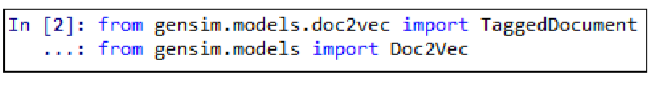
\includegraphics[width=4cm]{figures/1174096/tugas5/praktek3.PNG}
        \centering
        \caption{TaggedDocument dan Doc2Vec}
    \end{figure}

    \item Jelaskan dengan kata dan praktek cara menambahkan data training dari file yang dimasukkan kepada variabel dalam rangka melatih model doc2vac. 
    pertama tentukan terlebih dahulu tempat file dokumen tersebut disimpan kemudian import librari os setelah itu buat variabel unsup\_sentences yang berisikan array kosong, lalu tentukan file yang akan dimasukan setelah itu lakukan os listdir pada data yang akan dimasukan kemudian semua data tersebut di inisialisasi menjadi f kemudian nama f tersebut dimasukan ke variabel unsup. pada codingan tersebut merupakan praktikum untuk memasukan data doc2vec
    \begin{figure}[H]
        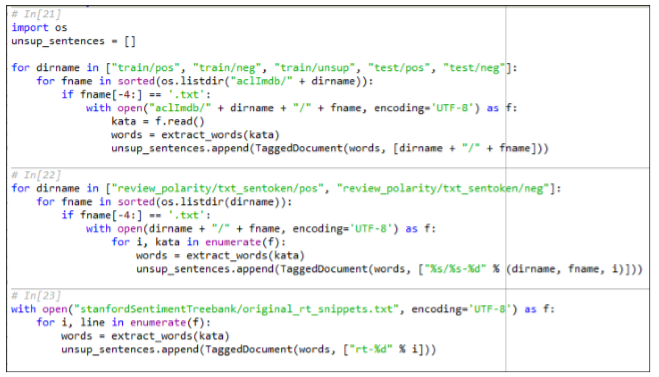
\includegraphics[width=4cm]{figures/1174096/tugas5/praktek4_1.PNG}
        \centering
        \caption{Data code}
    \end{figure}
    \begin{figure}[H]
        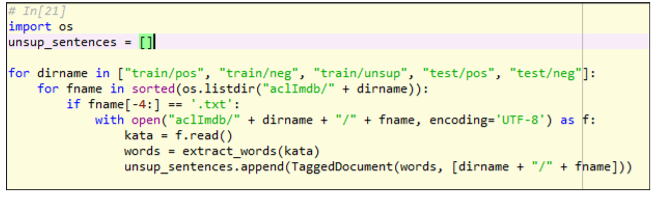
\includegraphics[width=4cm]{figures/1174096/tugas5/praktek4_2.PNG}
        \centering
        \caption{Data code}
    \end{figure}
    \begin{figure}[H]
        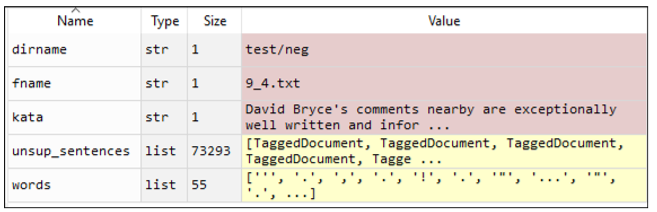
\includegraphics[width=4cm]{figures/1174096/tugas5/praktek4_3.PNG}
        \centering
        \caption{Data code}
    \end{figure}
    \begin{figure}[H]
        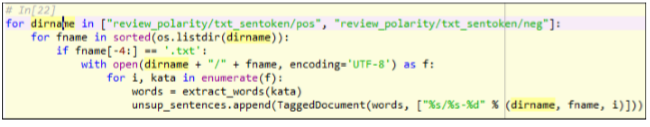
\includegraphics[width=4cm]{figures/1174096/tugas5/praktek4_4.PNG}
        \centering
        \caption{Data code}
    \end{figure}
    \begin{figure}[H]
        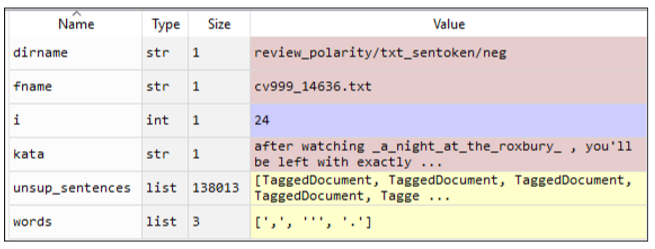
\includegraphics[width=4cm]{figures/1174096/tugas5/praktek4_5.PNG}
        \centering
        \caption{Data code}
    \end{figure}
    \begin{figure}[H]
        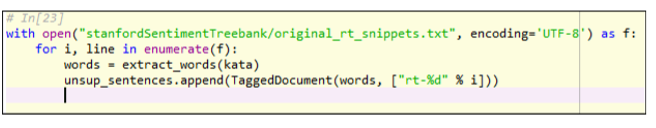
\includegraphics[width=4cm]{figures/1174096/tugas5/praktek4_6.PNG}
        \centering
        \caption{Data code}
    \end{figure}
    \begin{figure}[H]
        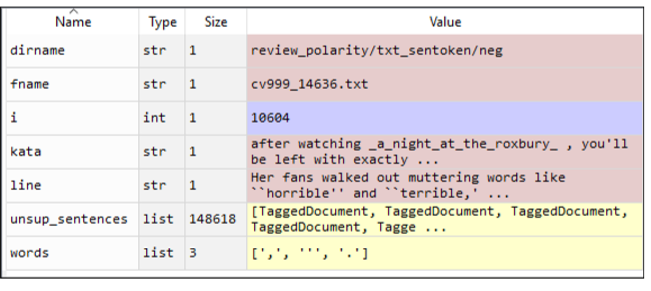
\includegraphics[width=4cm]{figures/1174096/tugas5/praktek4_7.PNG}
        \centering
        \caption{Data code}
    \end{figure}

    \item Jelaskan dengan kata dan praktek kenapa harus dilakukan pengocokan dan pembersihan data
    hal ini harus dilakukan supaya data lebih gampang untuk di olah dan meningkatkan tingkat akurasi dari proses pengolahan data Doc2Vec. kemudian harus dilakukan pembersihan data agar memori pc atau laptop yang di gunakan untuk mengolah data menjadi ringan dan menambah peforma dari mesin itu sendiri untuk codingan pertama lakukan terlebih dahulu rendomisasi. selanjutnya membuat variabel baru dengan nama mute yang di isi data class random dan data unsup\_sentence. kemudian setelah pengolahan data dilakukan pembersihan dengan melakukan code. 
    \hfill\break
    Proses pengocokan dan pembersihan data dilakukan dengan tahap melakukan shuffled dan randomisasi data, kemudian dibuat variabel untuk membuat data unsup\_senteces, lalu dibuat code untuk membersihkan data memory.
    \begin{figure}[H]
        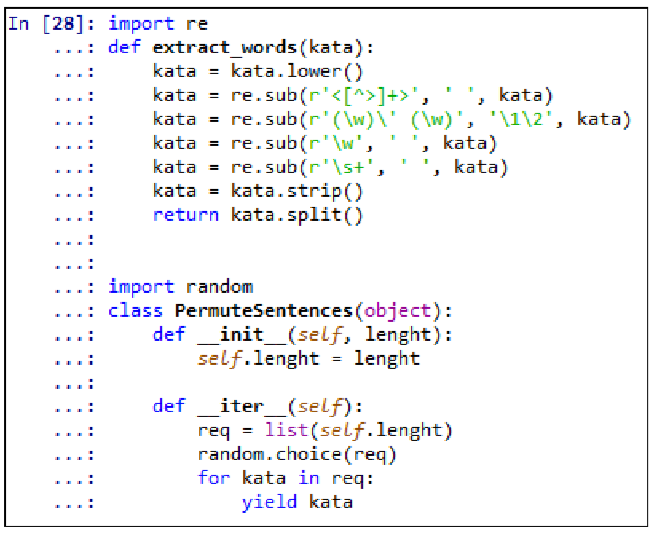
\includegraphics[width=4cm]{figures/1174096/tugas5/praktek5_1.PNG}
        \centering
        \caption{Shuffled dan Randomisasi data }
    \end{figure}
    \begin{figure}[H]
        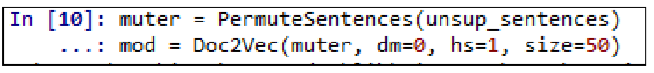
\includegraphics[width=4cm]{figures/1174096/tugas5/praktek5_2.PNG}
        \centering
        \caption{pembuatan variable muter untuk memuat data unsup\_sentences}
    \end{figure}
    \begin{figure}[H]
        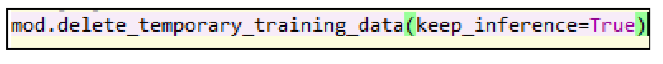
\includegraphics[width=4cm]{figures/1174096/tugas5/praktek5_3.PNG}
        \centering
        \caption{code untuk membersihkan data memory}
    \end{figure}

    \item Jelaskan dengan kata dan praktek kenapa model harus di save dan kenapa temporari training harus dihapus.
    Model Training harus disave supaya dalam pengolahan data tidak perlu menjalankan kembali data vektorisasi serta untuk meringankan beban ram. Selain itu temporary juga  harus dihapus guna meningkatkan peforma komputer.
    \begin{figure}[H]
        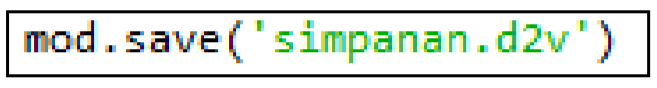
\includegraphics[width=4cm]{figures/1174096/tugas5/praktek6_1.PNG}
        \centering
        \caption{code untuk menyimpan data}
    \end{figure}
    \begin{figure}[H]
        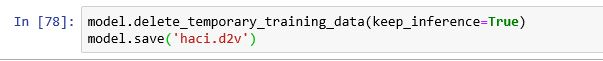
\includegraphics[width=4cm]{figures/1174096/tugas5/praktek6_2.JPG}
        \centering
        \caption{code untuk menghapus Temporary training}
    \end{figure}

    \item Jalankan dengan kata dan praktek maksud dari infer code.
    infer\_code digunakan untuk membandingkan data doc2vec yang telah di olah dengan kata yang baru atau data yang ada dalam perintah vector itu sendiri contoh membandingkan kata (i will go home). Kemudian untuk hasil running code tersebut terdapat hasil vektor yang rata rata berada pada kisaran 0,2 an yang berarti kata yang dimasukan pada inter\_vec datanya ada pada doc2vec atau ada data yang bobotnya menyamai kata-kata di dalam dokumen tersebut.
    \begin{figure}[H]
        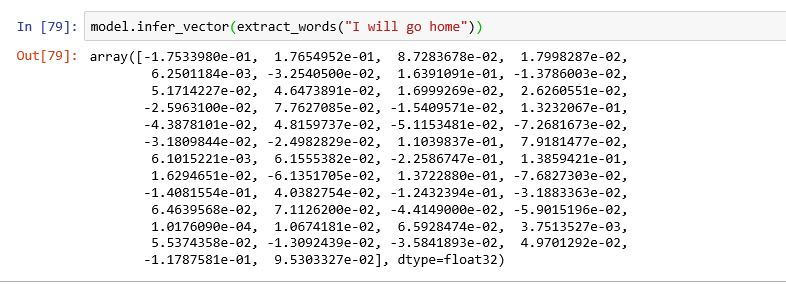
\includegraphics[width=4cm]{figures/1174096/tugas5/praktek7.JPG}
        \centering
        \caption{infer code}
    \end{figure}

    \item Jelaskan dengan praktek dan kata maksud dari cosine similarity
    Cosine Similarity merupakan sebuah algoritma yang digunakan untuk membandingkan dari dua buah data yang bukan merupakan data vector untuk menguji nilai kemiripan data satu dengan data lainnya. Setelah melakukan pengolahan data doc2vec dilakukan consine simirarity yang bertujuan untuk membandingkan data berisikan bahasa inggris dengan data yang telah di olah tadi apakah hasilnya mirip atau tidak.
    \begin{figure}[H]
        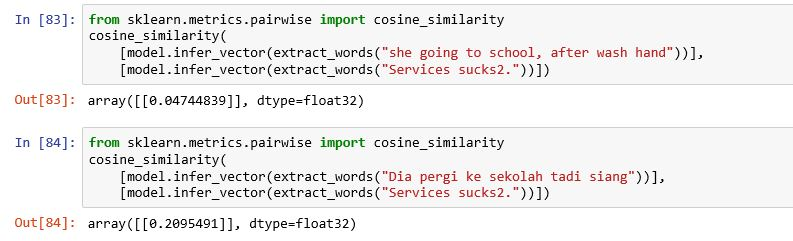
\includegraphics[width=4cm]{figures/1174096/tugas5/praktek8.JPG}
        \centering
        \caption{code Cosine Similarity}
    \end{figure}

    \item Jelaskan dengan praktek score dari cross validation masing-masing metode. 
    Ketika melakukan cross validation pertama masukan terlebih dahulu metode KNeighborsClasifier dan RandomForestClasifier dari library sklearn kemudian dilakukan cross validation setelah itu buat variabel clf dengan isi KNeighborsClasifier dan variabel clfrf dengan isi RandomForestClasifier kemudian di buat skor menggunakan cross validation dengan menggunakan variabel clf dan data sentvecs dan sentiments kemudian dengan numpy dibuat mean dari scores begitu pula untuk variabel clfrf selanjutnya melakukan import metode make\_pipeline yang dilakukan untuk membuat skor dari vektorisasi tfidf dan rf.
    \hfill\break
    Praktek cross validation dapat dilakukan dengan code berikut
    \lstinputlisting{src/1174096/5/1174096.py}
\end{enumerate}
    
\subsection{Penanganan Error}
\begin{enumerate}
	\item FileNotFoundError Error
	\begin{figure}[H]
		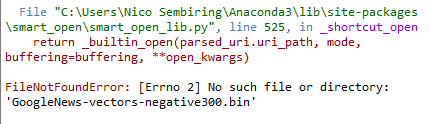
\includegraphics[width=4cm]{figures/1174096/tugas5/error.PNG}
		\centering
		\caption{FileNotFoundError}
	\end{figure}
	\item Tuliskan Kode Error dan Jenis Error
	\begin{itemize}
		\item FileNotFoundError
	\end{itemize}
	\item Cara Penangan Error
	\begin{itemize}
		\item FileNotFoundError
		\hfill\break
		Error terdapat pada kesalahan baca GoogleNews-vectors-negative300.bin yang tidak terbaca. Dikarenakan letak file yang dibaca tidak pada direktori yang sama. Seharusnya letakkan file di direktori yang sama. 
	\end{itemize}
\end{enumerate}
\subsection{Bukti Tidak Plagiat}
\begin{figure}[H]
\centering
	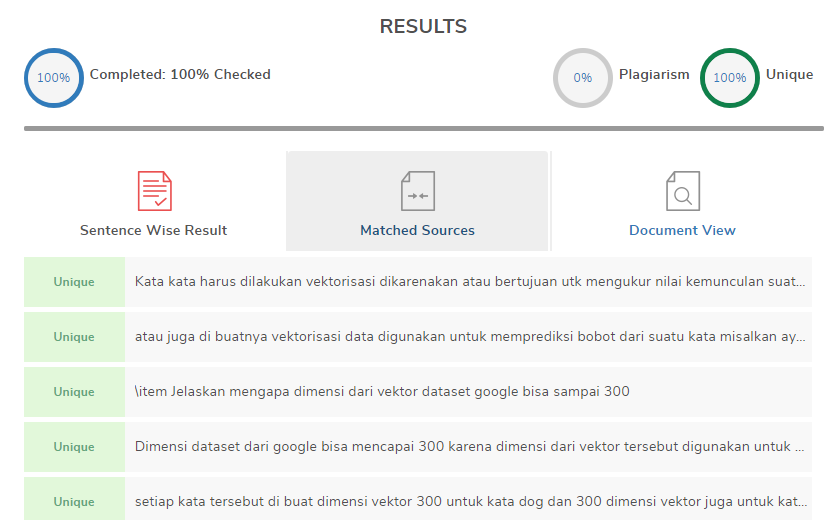
\includegraphics[width=4cm]{figures/1174096/tugas5/plagiarisme.PNG}
	\caption{Bukti Tidak Melakukan Plagiat Chapter 5}
\end{figure}
